\section{Implémentation}

\subsection{Vue d'ensemble}
\begin{figure}[h]
	\centering
	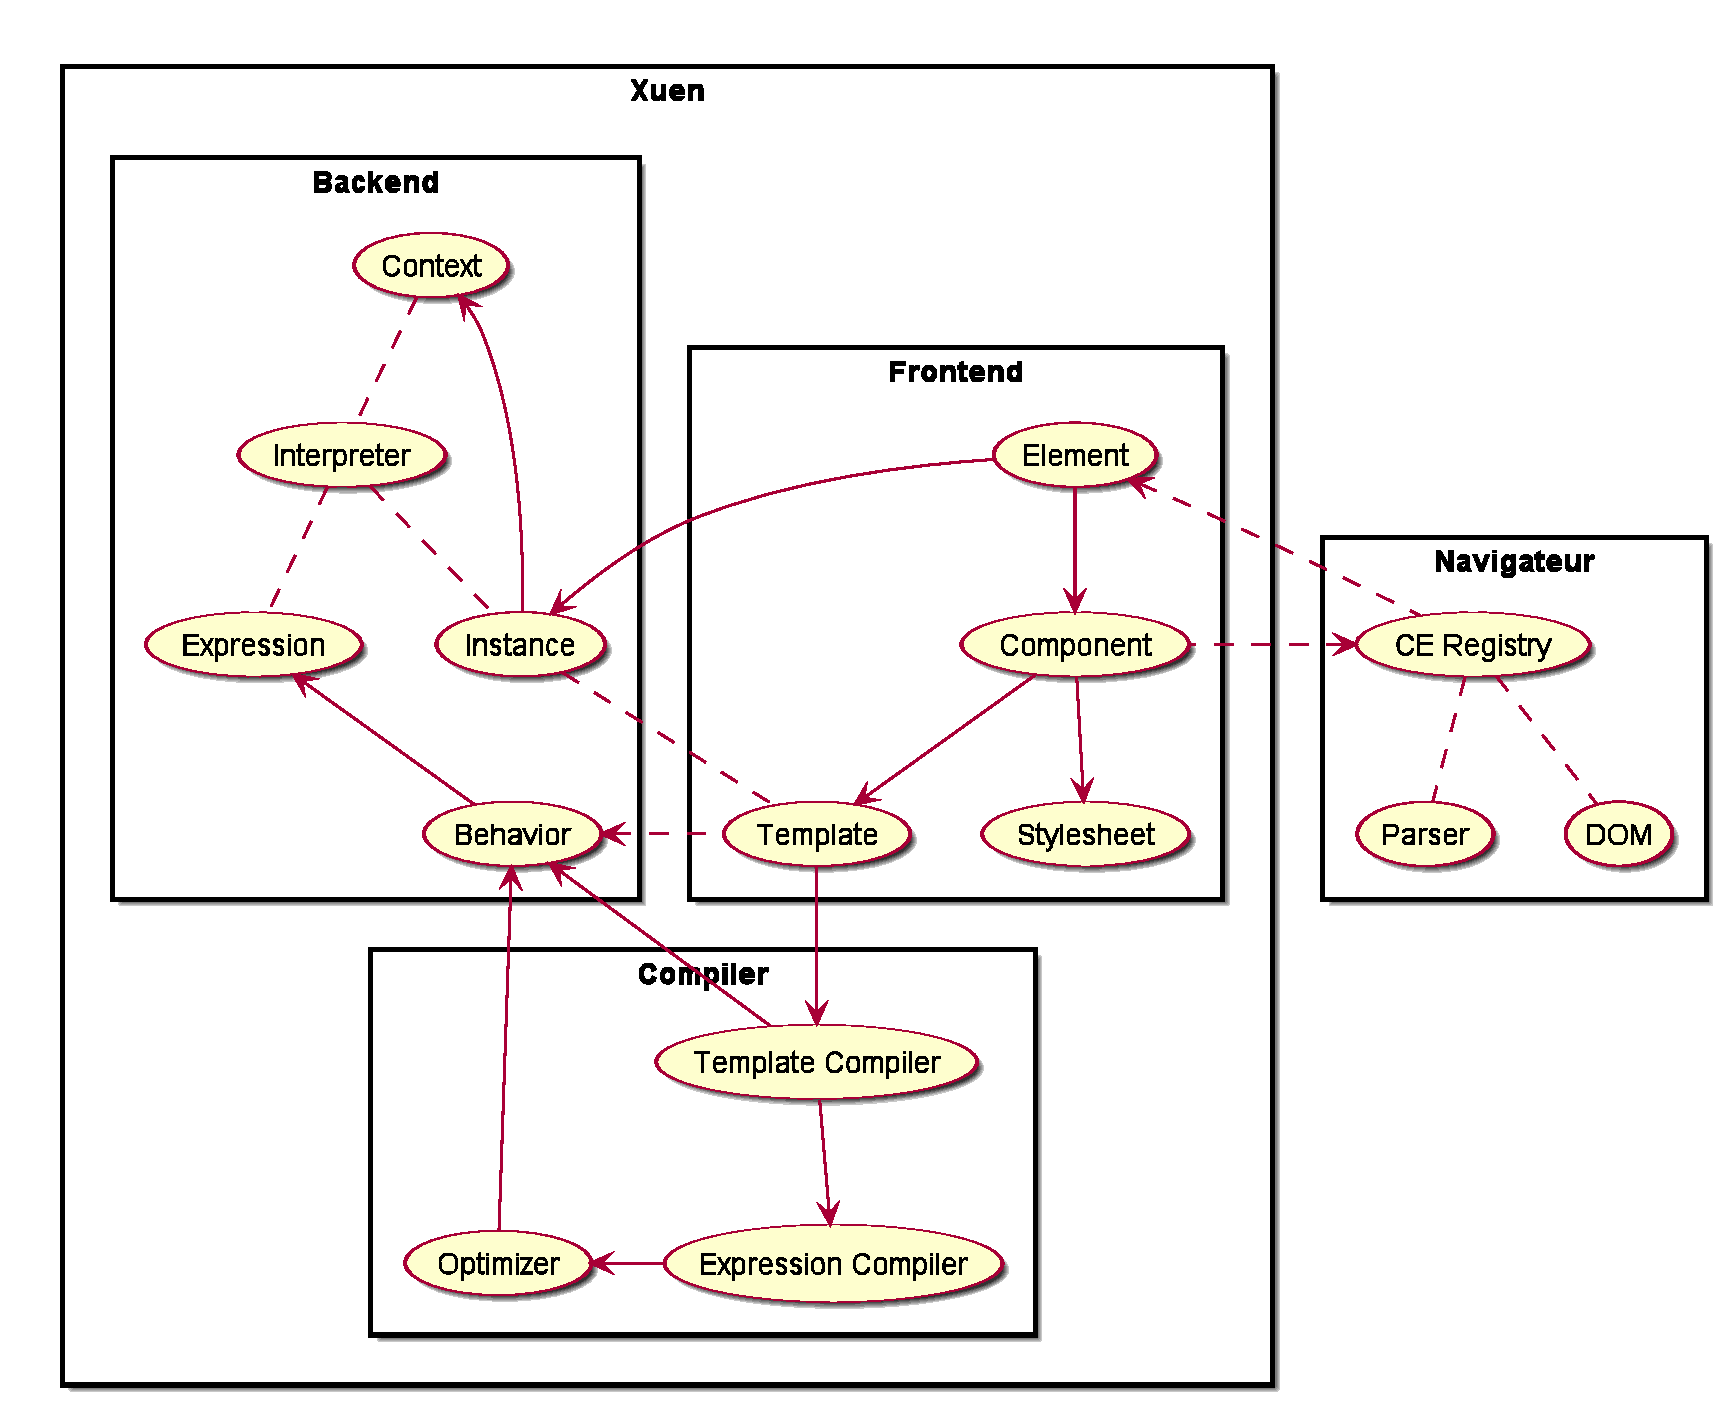
\includegraphics[width=\textwidth]{img/web_overview.eps}
	\caption{Vue d'ensemble de l'implémentation du framework Web}
	\label{fig:web-overview}
\end{figure}

L'implémentation du framework web de Xuen peut être décomposé en 3 grandes parties, tel qu'illustré par la figure \ref{fig:web-overview}.

\begin{enumerate}
	\item Le partie \emph{front-end} est exposée directement au développeur. Elle est utilisée pour déclarer les composants personnalisés de l'application, leurs comportements et structure.
	\item La partie \emph{back-end} est utilisée par le framework lorsqu'un élément est instancié dans le document. Elle fourni les outils nécessaire à l'implémentation des comportements dynamiques du template de cet élément et l'interface avec le système de signaux par le biais des expressions.
	\item Finalement le système de compilation est utilisé lors de la définition d'un nouveau composant pour transformer le code source HTML du template en une instance de la classe \texttt{Template}, encapsulant à la fois une structure pré-traitée du template, des modèles pour construire les comportements dynamique de ce template et des expressions sous forme d'arbres syntaxique prêt à être interprétés.  
\end{enumerate}

L'objectif de la partie de compilation est de réduire l'impact du traitement du template au \emph{runtime}. En effet, l'instanciation d'un template se base sur les outils fournis par le navigateur, notamment le parser HTML et son implémentation du DOM afin parcourir et traiter la structure fournie sous forme de code HTML.

En compilant le template et les expressions dès la déclaration, il n'est plus nécessaire de le faire lors de l'instanciation, ce qui permet un investissement fixe au chargement de l'application et des performances accrues lors de son fonctionnement.

Cette structure est en grande partie reprise d'un projet personnel antérieur. La plupart des éléments ont été repensés et réimplémentés, principalement pour les adapter au nouveaux standards \emph{Web Components} version \emph{v1} (par opposition à la version antérieur \emph{v0}). Le parser d'expression a quant à lui été récrit, passant d'une implémentation fortement inspirée du parser d'expression du framework Angular 2, mais en Scala, à une version développée avec la bibliothèque \emph{scala-parser-combinators} \cite{scala-parser-combinators}, plus propre et idiomatique. La grammaire du langage n'a cependant pas été significativement modifiée. L'optimisateur d'expressions est réutilisé pratiquement tel-quel.

\subsection{Processus de compilation du template}

Le template est fourni à la bibliothèque sous forme de code source HTML. La première opération consiste donc à construire dynamiquement un élément \texttt{<template>} et à y insérer le code du développeur. Le parser HTML du navigateur sera alors invoqué pour construire une structure de nœuds DOM. Cette structure est ensuite parcourue de façon récursive en commençant à l'élément template créé précédemment.

\begin{itemize}
	\item Premièrement, la nature du noeud en cours est déterminée. S'il s'agit d'un nœud \texttt{Text} ou \texttt{Comment}, son contenu est scanné pour y identifier d'éventuelles interpolations.
	\item Si le nœud est un élément, ses attributs sont observés.
	\item Si l'élément est annoté d'une transformation \texttt{*if} ou \texttt{*for}, cette transformation est appliquée.
	\item Si l'élément possède des annotations de \emph{data-binding}, celles-ci sont traitées.
	\item Les valeurs des attributs restants qui ne sont ni des transformations ni des annotations de \emph{data-binding} sont scannées pour y identifier des interpolations.
	\item Une fois l'élément lui-même entièrement traité, l'ensemble de ses enfants est parcouru, réitérant le processus.
\end{itemize}

Pour chaque nœud DOM devant être associé à un comportement dynamique, un \texttt{Behavior} est créé. Celui-ci est identifié par un numéro incrémenté à chaque nouvelle instance. Il sera de modèle pour la construction du comportement dynamique en question. Tous les \texttt{Behavior}s créés pour un template son rassemblé dans une \texttt{Map} contenue dans l'objet \texttt{Template} resultant. L'élément auquel le comportement doit être attaché est quant à lui décoré d'un attribut \texttt{xuen:behavior="..."} indiquant l'identifiant du comportement associé à ce nœud.

Si l'élément ne peut pas posséder d'attribut, c'est à dire lorsqu'il s'agit d'un nœud \texttt{Text} ou \texttt{Comment}, un élément \emph{placeholder} \texttt{<xuen:placeholder>} est inséré à sa place dans l'arbre DOM du template et l'attribut est placé sur cet élément. Dans ce cas, lors de la construction du comportement au moment de l'instanciation du template, l'élément \emph{placeholder} sera en premier lieu remplacé par un nœud correspondant à l'original puis le comportement spécifique de ce nœud sera implémenté.

Un \texttt{Behavior} peut en réalité implémenter plus d'un comportement pour un même élément. Si deux annotations sont présente sur un même élément, le \texttt{Behavior} construit à l'occasion du traitement de la première annotation est réutilisé pour la deuxième annotation. L'objet \texttt{Behavior} sera donc en charge de construire deux comportements dynamiques différents sur le même élément.

À l'inverse de la compilation, le processus d'instanciation est relativement simple. Le template est à présent sous forme normalisée, tous les comportements sont attachés à des éléments annoté par l'attribut \texttt{xuen:behavior}. Juste avant d'implémenter les comportement dynamiques, l'objet template est cloné pour construire une nouvelle structure indépendante de l'original qui est conservée en tant que modèle. La bibliothèque utilise alors la \texttt{Map} associant les identifiants des différents comportements enregistrés pour le template avec les objets \texttt{Behavior} encapsulant la logique de construction instancier à proprement parler ces comportements.

Le sélecteur css \texttt{[xuen:behavior="..."]} est utilisé pour récupérer l'élément sur lequel le comportement doit être appliqué puis la méthode \texttt{build} de l'objet \texttt{Behavior} est invoquée avec la référence vers l'élément courant. Cette méthode va alors instancier à proprement l'ensemble des comportements liés à cet élément.

De façon générale \emph{instancier un comportement} implique construire une paire signal + observateur qui implémentera le comportement désiré. Cette paire est initialement construite déconnectée. Une fois l'élément hôte connecté, son template est \emph{activé} ce qui entraine la liaison  des observateurs avec le signal associé et donc la mise en place du comportement dynamique.

Lorsqu'un élément est déconnecté, son template est \emph{désactivé}. Cette opération déconnecte l'ensemble des signaux et observateurs utilisé dans l'implémentation de ce template, assurant ainsi qu'il n'existe plus de lien entre le reste du système et l'élément déconnecté. Sans cette étape, il existe un risque que les éléments ne puissent pas être désalloués par le \emph{garbage collector} puisqu'une référence subsiste entre le reste du graphe de signaux et eux.

\subsection{Compilation des expressions}
\subsubsection{Optimisateur}
\subsection{Interprétation des expressions}

\newpage
\section{Difficultés rencontrées}
\subsection{Ordre de construction des \emph{custom elements}}

\textit{Cette section nécessite rédaction}

Pour résumer le problème: les éléments customs ne sont "upgradé" (le browser invoque le constructeur de la classe associée) que lorsqu'ils sont "connectés" (leur parent de niveau racine est un Document) SAUF s'il s'agit de l'élément parent étant instancié.

Le problème est que le callback \emph{connectedCallback} est invoqué sur l'élément parent avant que les éléments enfants ne soit considérés comme connectés et upgradés. Ainsi, lorsque le template de l'élément parent est activé avec la connexion au document, les éléments enfants n'ont même pas eu l'occasion de s'initialiser et les mécanismes de data-binding explosent.

La solution adoptée est de "monter" le template de l'élément premièrement dans un sous-enfant bidon du <body>, avant de le remonter correctement dans le sous-arbre DOM de l'élément. Ce passage rapide dans le body du document déclanche l'upgrade immédiat des éléments enfants, mais ajoute son lot de nouvelle complexités. L'élément enfant est en effet considéré comme "connecté" puis "déconnecté" au cours de l'initialisation de son parent, ce qui active le template de l'élément enfant avant que l'élément parent ait eu l'occasion de s'initialiser entièrement!! Afin de prévenir ce comportement, une variable globale \texttt{forcedUpgrade} est maintenue pour déterminer si la connexion d'un élément est lié à l'upgrade forcé ou non. Dans le cas où l'élément est connecté dans le but de l'upgrader, ses callbacks \texttt{connected} et \texttt{disconnected} sont ignorés.

Jusqu'à présent, cette solution semble fonctionner dans tous les cas. Ci-dessous l'ordre des opérations observées, avec le code de construction correspondant.

\begin{lstlisting}
class Foo extends Element(Foo)
object Foo extends Component[Foo](
	"x-foo", template = html"<x-bar><x-baz></x-baz></x-bar>",
	dependencies = List(Bar, Baz))

class Bar extends Element(Bar)
object Bar extends Component[Bar](
	"x-bar", template = html"<slot></slot>")

class Baz extends Element(Baz)
object Baz extends Component[Baz]("x-baz", template = html"Baz")
\end{lstlisting}

\subsubsection{Constructeur}
\begin{lstlisting}
val foo = new Foo
println("--")
dom.document.body.appendChild(foo)
\end{lstlisting}

\begin{lstlisting}
[x-foo] Upgrade start
[x-foo] Upgrade end
--
[x-foo] Connected
[x-bar] Upgrade start
[x-bar] Upgrade end
[x-bar] Connected
[x-baz] Upgrade start
[x-baz] Upgrade end
[x-baz] Connected
\end{lstlisting}

\subsubsection{Parser HTML (connecté)}
\begin{lstlisting}
dom.document.body.innerHTML = "<x-foo></x-foo>"
\end{lstlisting}

\begin{lstlisting}
[x-foo] Upgrade start
[x-bar] Upgrade start
[x-bar] Upgrade end
[x-bar] Connected
[x-baz] Upgrade start
[x-baz] Upgrade end
[x-baz] Connected
[x-foo] Upgrade end
[x-foo] Connected
\end{lstlisting}


\subsubsection{Parser HTML (déconnecté)}
\begin{lstlisting}
val div = dom.document.createElement("div")
div.innerHTML = "<x-foo></x-foo>"
\end{lstlisting}

\begin{lstlisting}
[x-foo] Upgrade start
[x-foo] Upgrade end
\end{lstlisting}